\documentclass[12pt,titlepage]{article}
\usepackage[table]{xcolor}
\usepackage{longtable}
\usepackage[utf8]{inputenc}
%Language of Document Elements like Figure or Table
\usepackage[english]{babel}
\usepackage[bookmarks]{hyperref}
\usepackage{pdfpages}
\usepackage{graphicx}
\usepackage{float}
\usepackage{array}
\usepackage{lipsum} 
\usepackage[justification=centering]{caption}
\usepackage{enumitem}
\usepackage{chngcntr}
\usepackage{lscape}
\usepackage{fancyhdr}
\usepackage{listings}
\usepackage[style=alphabetic, backend=biber]{biblatex}
\usepackage{dafny}
\usepackage{hyperref}
\usepackage{nameref}
\usepackage[margin=1in]{geometry}

%Each Section in a new Page
\let\oldsection\section
\renewcommand\section{\clearpage\oldsection}

%Set space around and between lists
\setlist[enumerate]{noitemsep, topsep=0cm}
\setlist[itemize]{noitemsep, topsep=0cm}

%Figure/Table Numbering style "Section Number.figure counter
\renewcommand{\thefigure}{\arabic{section}.\arabic{figure}}
\renewcommand{\thetable}{\arabic{section}.\arabic{table}}

%Reset figure/table counter after section change
\counterwithin{figure}{section}
\counterwithin{table}{section}

%Syntax Highlighting
%\lstdefinestyle{dafny}{
%	language=dafny, 
%	basicstyle=\normalfont\ttfamily,
%	numbers=left,
%	numberstyle=\scriptsize,
%	stepnumber=1,
%	numbersep=8pt,
%	showstringspaces=false,
%	breaklines=true,
%	frame=lines,
%	backgroundcolor=\color{background}
%}

\colorlet{punct}{red!60!black}
\definecolor{background}{HTML}{EEEEEE}
\definecolor{delim}{RGB}{20,105,176}
\colorlet{numb}{magenta!60!black}

\lstdefinelanguage{json}{
	basicstyle=\normalfont\ttfamily,
	numbers=left,
	numberstyle=\scriptsize,
	stepnumber=1,
	numbersep=8pt,
	showstringspaces=false,
	breaklines=true,
	frame=lines,
	backgroundcolor=\color{background},
	literate=
	*{0}{{{\color{numb}0}}}{1}
	{1}{{{\color{numb}1}}}{1}
	{2}{{{\color{numb}2}}}{1}
	{3}{{{\color{numb}3}}}{1}
	{4}{{{\color{numb}4}}}{1}
	{5}{{{\color{numb}5}}}{1}
	{6}{{{\color{numb}6}}}{1}
	{7}{{{\color{numb}7}}}{1}
	{8}{{{\color{numb}8}}}{1}
	{9}{{{\color{numb}9}}}{1}
	{:}{{{\color{punct}{:}}}}{1}
	{,}{{{\color{punct}{,}}}}{1}
	{\{}{{{\color{delim}{\{}}}}{1}
	{\}}{{{\color{delim}{\}}}}}{1}
	{[}{{{\color{delim}{[}}}}{1}
	{]}{{{\color{delim}{]}}}}{1},
}


%TODO
\newcommand{\todonl}[1]{\newline\textcolor{red}{TODO: #1}\PackageWarning{TODO:}{#1!}}
\newcommand{\todo}[1]{\textcolor{red}{TODO: #1}\PackageWarning{TODO:}{#1!}}

%Set Paragraph indent to null
\setlength{\parindent}{0pt}
% Smaler Table Space
\renewcommand{\arraystretch}{1.5}

\title{Visual Studio Code Integration for the Dafny Language and Program Verifier}
\author{Rafael Krucker, Markus Schaden}
\date{20.02.2017}

\pagestyle{fancy}
\lhead{BA Dafny}
\addbibresource{LITERATURVERZEICHNIS/bibliographie.bib}
\begin{document}
\pagenumbering{Roman} 

% TODO
%
\includepdf{titlepage/titlepage}

% TODO
%\phantomsection
\addcontentsline{toc}{section}{Abstract}
\section*{Abstract}
[Placeholder Abstract Text]
%\newpage
%\phantomsection
\addcontentsline{toc}{section}{Management Summary}
\section*{Management Summary}
\subsection*{Ausgangslage}
[Placeholder]

\subsection*{Vorgehen}
[Placeholder]

\subsection*{Technologien}
[Placeholder]

\subsection*{Ergebnisse}
[Placeholder]

\subsection*{Ausblick}
[Placeholder]


% TODO
%\includepdf[pages={1-}, 
%scale=0.9,pagecommand=\thispagestyle{plain}]{additionals/eigenstaendigkeit}
%\includepdf[pages={1-2}, 
%scale=0.9,pagecommand=\thispagestyle{plain}]{additionals/aufgabenstellung}

\newpage
\tableofcontents
\newpage
\pagenumbering{arabic}
\section{Outline}
\subsection{The problem and its setting}
This chapter presents the background of the study, problem and its significance, and the scope and deliminition of the study.
\subsubsection{Introduction}
Dafny is a language designed and implemented by Microsoft Research. It offers built-in specification constructs. These include pre- and postconditions, frame specifications as well as termination metrics. Further support such as ghost variables and recursive functions are also implemented. Through such specification primitives, the Dafny verifier, invoked during compilation, can be used to verifiy the specified aspects of the functional correctness of the program. \newline
Dafny is typically used via its Visual Studio  IDE integration under the Windows operating system. Dafny can be run from the command line and a Visual Studio integration exists. The This integration verifier therefor allows for an efficient workflow of editing a program while constantly being given feedback about its the functional correctness. The Dafny compiler and verifier can additionally be invoked from the command line. \newline
Microsoft would like to integrate of Dafny into the cross-platform Visual Studio Code IDE. Work on this has already been started through a plugin by Jonathan  Rionatan. It currently works within the mono-environment and provides feedback from the verifier. \newline

\subsubsection{Statement of the problem}
This thesis aimes to research on how Dafny programmers can be best supported during their work and incorporate these findings in a production quality plugin for Visual Studio Code. 
\subsubsection{Significance of study}
Since the goal of the thesis is a production quality plugin, the thesis aims to immidiately simplify the way programmers use Dafny. Through Dafny's strong functional correctness facilities and Visual Studio Code's simple and modular architecture there is a chance that the plugin could guide developers through the transition to world of multi-core and multi-threaded applications, which are becoming more and more popular. Also in high risk domains the use of a specification constructs is of great benefit for the developers, which the developed plugin aims to make easier to harvest.
\subsubsection{Scope and delimination}
The plugin is limited to be used in three defined environments, although they compromise a huge percentage of environments used in programming. The plugin offers a fixed set of features which are detailed in this thesis, but remains open for adaption and extension.
\subsubsection{Definition of terms}

\section{Use Cases}
\subsection{Use Case Diagram}
\begin{figure}[h]
	\centering
	\includegraphics[width=1\linewidth, height=5in]{"./img/UseCase"}
	\caption{Use Case Diagram}
	\label{fig:usecase-diagram}
\end{figure}
\subsection{Actors and Stakeholder}
\begin{itemize}
	\item Programmers
	\item Microsoft
\end{itemize}
\subsection{Descriptions (brief)}
\subsubsection{UC1: Windows Installation}
A programmer can install the Dafny Plugin on his .Net environment running on Windows 10.
\subsubsection{UC2: Linux Installation}
A programmer can install the Dafny Plugin on his mono environment running on a common Linux distribution such as Ubuntu 16.04.
\subsubsection{UC3: OSX Installation}
A programmer can install the Dafny Plugin on his mono environment running on OSX ??? (VERSION).
\subsubsection{UC4: Easy installation of Dafny plugin}
A programmer can simply install the Dafny plugin by running an automatic installer which sets all path variables and makes additional needed environment adjustments.
\subsubsection{UC5: Syntax Highlighting}
The system automatically does syntax highlighting while the user writes a Dafny (dfy.) file.
\subsubsection{UC6: Reporting of Dafny best practices violations}
The plugin can be configured with a simple DSL config file which describes common best practices for Dafny. The plugin reports violations of these rules via the standard Visual Studio Code notification mechanisms.
\subsubsection{UC7: Automatic generation of contracts}
The plugin can be configured with a simple DSL-File to recognize certain semantics, which could benefit from the setting of Pre- and Postconditions. The plugin offers to add these in form of a refactoring via the common Visual Studio Code mechanisms.
\subsubsection{UC8: Autocompletion for identifiers}
The plugin offers autocompletion of Dafny code while the user types via the standard Visual Studio Code mechanisms.
\subsection{Descriptions (fully dressed)}
\subsubsection{UC1: Windows Installation}
\rowcolors{1}{gray!25}{white}
\begin{longtable}{l | p{0.7\textwidth} }
	Description & A programmer can install the Dafny Plugin on his .Net environment running on Windows 10.\\ \hline
	Primary Actor & Programmer\\ \hline
	Trigger & Programmer wants to programm Dafny in Visual Studio Code.\\ \hline
	Stakeholder and Interests & 
	\begin{itemize}
		\item Programmer: Wants stable support from the IDE while developing Code.
		\item Microsoft: Wants a stable Dafny integration to fulfill the needs of its clients.
	\end{itemize} \\ \hline
	Preconditions & 
 \begin{itemize}
		\item Windows 10 Environment with a modern version of the .Net Framework installed.
	\end{itemize} \\ \hline
	Postconditions & 
	\begin{itemize}
		\item The plugin works without problems, the programmer can start writing code.
	\end{itemize} \\ \hline
	Main Success Scenario & 1. Programmer downloads the plugin. \newline
	2. During an automated installation routine, the plugin installs itself and all needed environmental changes are made. (UC4) \newline
	3. Visual Studio code is updated to use the plugin, a success message is shown\\ \hline
	Extensions & 
	2a. The installer notices that some dependencies are missing. \newline 
	- It notifies the programmer accordingly.\\ \hline
	Special Requirements & None\\ \hline
	Frequency of Occurence & Usually once per working environment\\ \hline
	Open Issues & None \\ \hline
	\caption{UC1}
\end{longtable}
\subsubsection{UC2: Linux Installation}
\begin{longtable}{l | p{0.7\textwidth} }
	Description & A programmer can install the Dafny Plugin on his mono environment running on a common Linux distribution such as Ubuntu 16.04.\\ \hline
	Primary Actor & Programmer\\ \hline
	Trigger & Programmer wants to programm Dafny in Visual Studio Code.\\ \hline
	Stakeholder and Interests & 
	\begin{itemize}
		\item Programmer: Wants stable support from the IDE while developing Code.
		\item Microsoft: Wants a stable Dafny integration to fulfill the needs of its clients.
	\end{itemize} \\ \hline
	Preconditions & 
	\begin{itemize}
		\item A modern common Linux distribution such Ubuntu 16.04 or Fedora with the mono framework installed.
	\end{itemize} \\ \hline
	Postconditions &
	\begin{itemize}
		\item The plugin works without problems, the programmer can start writing code.
	\end{itemize} \\ \hline
	Main Success Scenario &
	1. Programmer downloads the plugin. \newline
	2. During an automated installation routine, the plugin installs itself and all needed environmental changes are made. (UC4) \newline
	3. Visual Studio code is updated to use the plugin, a success message is shown\\ \hline
	Extensions &
	2a. The installer notices that some dependencies are missing. \newline
	- It notifies the programmer accordingly.\\ \hline
	Special Requirements & None\\ \hline
	Frequency of Occurence & Usually once per working environment\\ \hline
	Open Issues & None \\ \hline
	\caption{UC2}
\end{longtable}

\subsubsection{UC3: OSX Installation}
\begin{longtable}{l | p{0.7\textwidth} }
	Description & A programmer can install the Dafny Plugin on his mono environment running on OSX.\\ \hline
	Primary Actor & Programmer\\ \hline
	Trigger & Programmer wants to programm Dafny in Visual Studio Code.\\ \hline
	Stakeholder and Interests & 
	\begin{itemize}
		\item Programmer: Wants stable support from the IDE while developing Code.
		\item Microsoft: Wants a stable Dafny integration to fulfill the needs of its clients.
	\end{itemize} \\ \hline
	Preconditions &
	\begin{itemize}
		\item A modern version of the OSX OS installed such as canberra with the mono framework installed.
	\end{itemize} \\ \hline
	Postconditions &
	\begin{itemize}
		\item The plugin works without problems, the programmer can start writing code.
	\end{itemize} \\ \hline
	Main Success Scenario & 1. Programmer downloads the plugin. \newline
	2. During an automated installation routine, the plugin installs itself and all needed environmental changes are made. (UC4) \newline
	3. Visual Studio code is updated to use the plugin, a success message is shown\\ \hline
	Extensions & 
	2a. The installer notices that some dependencies are missing. \newline 
	- It notifies the programmer accordingly.\\ \hline
	Special Requirements & None\\ \hline
	Frequency of Occurence & Usually once per working environment\\ \hline
	Open Issues & None \\ \hline
	\caption{UC3}
\end{longtable}

\subsubsection{UC4: Easy installation of Dafny plugin}
\begin{longtable}{l | p{0.7\textwidth} }
	Description & A programmer can simply install the Dafny plugin by running an automatic installer which sets all path variables and makes additional needed environment adjustments.\\ \hline
	Primary Actor & Programmer\\ \hline
	Trigger & Programmer wants install the Dafny plugin to visual studio code.\\ \hline
	Stakeholder and Interests & Programmer: Wants an easy, automated installation of the plugin. \newline Microsoft: Wants a stable Dafny integration to fulfill the needs of its clients.\\ \hline
	Preconditions &\begin{itemize}
		\item Depending on the environment, the preconditions of UC1, UC2 or UC3 are satisfied.
		\item Visual Studio Code is installed.
		\item The programmer has admin priviledges in his environment.
	\end{itemize}\\ \hline
	Postconditions & 
	\begin{itemize}
		\item The plugin works without problems, the programmer can start writing code.
	\end{itemize} \\ \hline
	Main Success Scenario & 
	1. Programmer downloads the plugin via the Visual Studio Code plugin store. \newline
	2. The plugin determines which platform it is run on, and sets either the path to the .Net framework or the mono framework. \newline
	3. The plugin downloads the Dafny and sets the path to the Dafny server binary. \newline
	4. The plugin then installs itself via the standard Visual Studion Code plugin mechanisms. \newline
	5. The plugin prompts a success message and the programmer is ready to code in Dafny.\\ \hline
	Extensions & 
	2a. The installer can't find, depending on the enviroment, either the mono or the .Net framework in the standard locations. \newline 
	- It prompts the user to enter the location and does so until the framework is found. \\ \hline
	Special Requirements & None\\ \hline
	Frequency of Occurence & Usually once per working environment\\ \hline
	Open Issues & None \\ \hline
	\caption{UC4}
\end{longtable}

\subsubsection{UC5: Syntax Highlighting}
\begin{longtable}{l | p{0.7\textwidth} }
	Description & The system automatically does syntax highlighting while the user writes a Dafny (dfy.) file.\\ \hline
	Primary Actor & Programmer\\ \hline
	Trigger & Programmer writes Dafny code in Visual Studio Code.\\ \hline
	Stakeholder and Interests & Programmer: Wants enhanced readability for the source files he's working on. \newline Microsoft: Wants a state of the art IDE integration of Dafny.\\ \hline
	Preconditions &
	\begin{itemize}
		\item Visual Studio Code with the Dafny plugin installed is running.
		\item Dafny code is being written in a .dfy file.
	\end{itemize}\\ \hline
	Postconditions &
	\begin{itemize}
		\item The source code is highlighted in different colors according to common standards in general and the Visiual Studio Code guidelines specifically.
	\end{itemize}\\ \hline
	Main Success Scenario & 
	1. Programmer types code into a .dfy file. \newline
	2. The plugin detects the changes and applies syntax highighlighting through the standard Visual Studio Code mechanisms.\\ \hline
	Extensions & 
	2a. The newly written code causes a compilation error and cannot be interpreted. \newline 
	- The previous syntax highlighting stays in place, the errors are highlighted according to common practices with compilation errors in Visual Studio Code. \\ \hline
	Special Requirements & None\\ \hline
	Frequency of Occurence & Very often, after every key up event.\\ \hline
	Open Issues & None \\ \hline
	\caption{UC5}
\end{longtable}

\subsubsection{UC6: Reporting of Dafny best practices violations}
\begin{longtable}{l | p{0.7\textwidth} }
	Description & The plugin can be configured with a simple DSL config file which describes common best practices for Dafny. The Plugin reports violations of these rules via the standard Visual Studio Code notification mechanisms.\\ \hline
	Primary Actor & Programmer\\ \hline
	Trigger & Programmer writes Dafny code in Visual Studio Code.\\ \hline
	Stakeholder and Interests & Programmer: Wants to write the cleanest code possible using common Dafny idioms. \newline Microsoft: Wants to support programmers getting the most out of Dafny.\\ \hline
	Preconditions &
	\begin{itemize}
		\item Visual Studio Code with the Dafny plugin installed is running.
		\item Dafny code is being written in a .dfy file.
	\end{itemize}\\ \hline
	Postconditions &
	\begin{itemize}
		\item Violations of common best practices for Dafny are reported through the standard Visual Studio Code mechanisms.
	\end{itemize}\\ \hline
	Main Success Scenario & 
	1. The plugin is installed preconfigured with a collection of common best practives for Dafny, which is done through a DSL file. \newline
	2. Programmer types code into a .dfy file. \newline 
	3. The plugin continuously checks for violations of the rules. \newline 
	4. If a violation is detected, it is reported through the standard mechanisms of Visual Studio Code.\\ \hline
	Extensions & 
	1a. The predefined rules are not sufficient for the programmer. \newline 
	- The programmer can updated the configuration file himself to include his own or his company's coding guidelines. \\ \hline
	Special Requirements & None\\ \hline
	Frequency of Occurence & Very often, after new valid syntax was written.\\ \hline
	Open Issues & None \\ \hline
	\caption{UC6}
\end{longtable}

\subsubsection{UC7: Automatic generation of contracts}
\begin{longtable}{l | p{0.7\textwidth} }
	Description & The plugin can be configured with a simple DSL-File to recognize certain semantics, which could benefit from the setting of Pre- and Postconditions. The plugin offers to add these in form of a refactoring via the common Visual Studio Code mechanisms.\\ \hline
	Primary Actor & Programmer\\ \hline
	Trigger & Programmer writes Dafny code in Visual Studio Code.\\ \hline
	Stakeholder and Interests & Programmer: Wants to write the correctest code possible making use of Dafny's specification constructs. \newline Microsoft: Wants to support programmers getting the most out of Dafny.\\ \hline
	Preconditions &
	\begin{itemize}
		\item Visual Studio Code with the Dafny plugin installed is running.
		\item Dafny code is being written in a .dfy file.
	\end{itemize}\\ \hline
	Postconditions &
	\begin{itemize}
		\item Specification constructs suitable for the context were added as refactorings.
	\end{itemize}\\ \hline
	Main Success Scenario & 
	1. The plugin is installed preconfigured with a collection of common semantics for Dafny and their corresponding specification constraints, which is done through a DSL file. \newline
	2. Programmer types code into a .dfy file. \newline 
	3. The plugin continuously checks for semantics that could benefit form the setting of specification constraints. \newline 
	4. If such a semantic is detected, it is reported through the standard mechanisms of Visual Studio Code, with a refactoring offered to add the constraints. \newline
	5. The programmer invokes the refactorings and the necessary code is added.\\ \hline
	Extensions & 
	1a. The predefined semantics and refactorings are not sufficient for the programmer. \newline 
	- The programmer can updated the configuration file himself to include support for his own or his company's  common code semantics. \\ \hline
	Special Requirements & None\\ \hline
	Frequency of Occurence & Very often, after new valid syntax was written.\\ \hline
	Open Issues & None \\ \hline
	\caption{UC7}
\end{longtable}

\subsubsection{UC8: Autocompletion for identifiers}
\begin{longtable}{l | p{0.7\textwidth} }
	Description & The plugin offers autocompletion of Dafny code while the user types via the standard Visual Studio Code mechanisms.\\ \hline
	Primary Actor & Programmer\\ \hline
	Trigger & Programmer writes Dafny code in Visual Studio Code.\\ \hline
	Stakeholder and Interests & Programmer: Wants enhanced productivity while writing Dafny code. \newline Microsoft: Wants a state of the art IDE integration of Dafny.\\ \hline
	Preconditions &
	\begin{itemize}
		\item Visual Studio Code with the Dafny plugin installed is running.
		\item Dafny code is being written in a .dfy file.
	\end{itemize}\\ \hline
	Postconditions &
	\begin{itemize}
		\item An identifier was autocompleted.
	\end{itemize}\\ \hline
	Main Success Scenario & 
	1. Programmer types code into a .dfy file. \newline
	2. The plugin detects the changes and searches for the beginning of known identifiers. \newline
	3. If such a beginning is found, completion if offered through the standard mechanisms of Visual Studio Code.\\ \hline
	Extensions & 
	None. \\ \hline
	Special Requirements & None\\ \hline
	Frequency of Occurence & Very often, after every key up event.\\ \hline
	Open Issues & None \\ \hline
	\caption{UC8}
\end{longtable}
\section{Project management}
\subsection{Projectplan}
\begin{figure}[H]
	\centering
	\includegraphics[width=1.2\textwidth]{img/projectplan}
	\caption{Projectplan}
	\label{fig:Projectplan}
\end{figure}
\subsection{Milestones}
\rowcolors{1}{gray!25}{white}
\begin{longtable}[H]
	{l| l | p {0.7\textwidth}}
	\textbf{Nr} & \textbf{Title} & \textbf{Description} \\ 
	\hline\hline
	
	M1 & First prototype & Plugin is working on all operation systems, simple verification is in place and errors are reported, basic syntax highlighting \\ 
	
	M2 & Improved prototype & Automatic downloading of dependencies and installation of Dafny and configure of environment variables \\ 
	
	M3 & Contract generation & First automatic contract generation, customizable with DSL \\ 
	
	M4 & Autocompletion & Autocompletion for identifiers \\ 
	
	M5 & Release 1.0 & Everything implemented and tested. Ready to be published \\ 		
	\caption{Milestone}
	\label{tab:Milestone}
\end{longtable}
\subsection{Risk management}
\begin{landscape}
	\rowcolors{2}{gray!25}{white}
	\begin{longtable}[H]
		{l|p{0.22\textwidth}| p{0.22\textwidth} | p{0.1\textwidth} | p{0.1\textwidth} | p{0.25\textwidth} | p{0.25\textwidth}}
		
		\textbf{Nr} & \textbf{Title} & \textbf{Description} & 
		\textbf{Max Harm [h]} & \textbf{Proba- bility} & \textbf{Prevention} &  
		\textbf{Behaviour at entry}\\ \hline
		
		R1 & Underestimation of workload & One or more team members can't finish a feature in time or loses to much time on a minor feature & 120 & 25\% & Weekly scrum meetings with feedback about the current work progress. Estimate workload together. Include time reserve & Help each other, if one is struggling. Feature reduction as last resort. \\ 
		
		R2 & Workflow is not working & Toolchain is not working as planed. The used components aren't ideal for the problem & 30 & 15\% & Use experience to get a good setup and test it alot in the beginning & Redefine toolchain or change single tool \\ 
		
		R3 & Communication problems & Team is not working together and each member is developing individually. Creation of incompatible interfaces. Talking with the industrial partner isn't possible as expected, due to time difference or not enough time & 70 & 20\% & Weekly scrum meetings and agreements. Already worked in other projects as a team before & Increase written documentation and working closer together. Having a fixed meeting with the industrial partner \\ 
		
		R4 & Lack of knowledge & Team has to little knowledge about Dafny, VSCode and the development of a VSCode Plugin & 80 & 10\% & Already experience with typescript for plugin development, as preparatory work informed about Dafny & Find necessary knowledge online, get help from Microsoft Research \\ 
		
		R5 & Data loss or manipulation & Data loss because of a server crash or open permissions to access and modify data & 20 & 3\% & Regularly backups and restrictive permissions to change files & Use backup to restore data. Extend safety measures \\ 
		
		R6 & Failure developer machine & One of the developer machines isn't working anymore. & 10 & 1\% & Limited, regularly commits and backups. & Switch temporary to the school computer and install the necessary tools. \\
		
		R7 & Implementing the DSL is too complicated or too difficult to use & The DSL would be needed to suggest possible contracts or to customize the best practices. & 100 & 30\% & This core feature has to be researched carefully so that it really fits our needs and that other developers can really use the plugin. & Read about DSL, talking to people which have already worked with it. \\
		
		R8 & Supporting all features on the different environments is not possible & Due to that Windows, OSX and Linux are quite different, it could be that some features aren't possible to implement on a platform or causes a big overhead to get it running & 10 & 25\% & Using as much of the standard API as possible. Implement specific features platform dependant. & Disable a certain feature on a platform or look for a workaround. \\	
		
		R9 & Automatic installer of Dafny is not possible & Maybe because of security restrictions, it could be possible that you can't download and install additional software and set environment variables. & 35 & 20\% & Test if downloading of software can done inside VS Code. & Automatic installer can't be done inside the plugin. Switch to a different strategy and implement an automatic installer over a additional executable, which could also install the plugin in vscode. \\
		
		\caption{Risk management}
		\label{tab:Risk management}
	\end{longtable}
\end{landscape}

\subsection{Risk Matrix}
\begin{figure}[H]
	\centering
	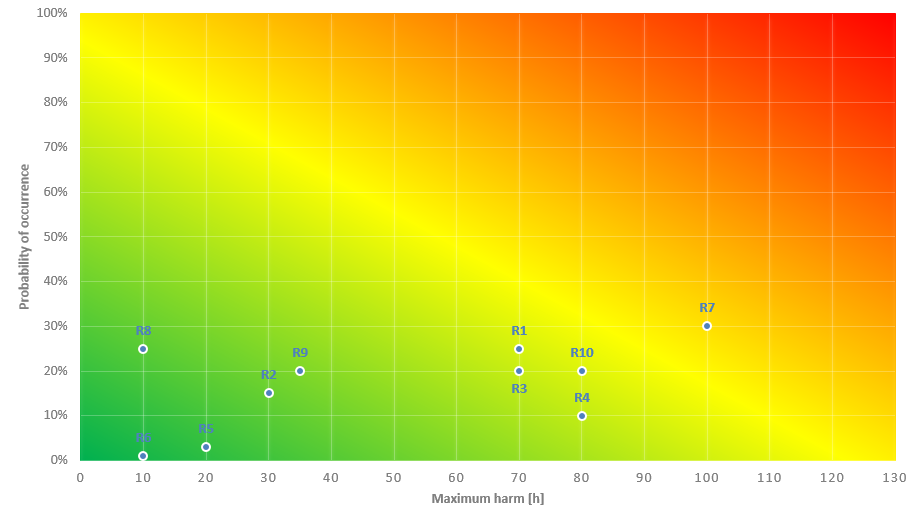
\includegraphics[width=1\textwidth]{img/riskmatrix}
	\caption{Risk Matrix}
	\label{fig:Risk Maxtrix}
\end{figure}
\section{Systemsetup}
\subsection{Local setup}
TexStudio 2.12\newline
Visual Studio Code 1.9\newline
Git 


\subsection{Server setup}
Jira \newline
Bamboo\newline
NodeJS\newline
SonarQube\newline
Postgres


\subsection{Continuous Integration}

To ensure that the code quality is high and the code is working as expected, all commits trigger automated builds of the respective project. A commit to the documentation repository executes a job which creates a pdf out of the latex sources. This document is then copied to the wwwroot directory, which then can be downloaded from the project homepage. Commits to the vscode-dafny repository will result in a build and a complete run of all tests on the three environments afterwards. Therefore remote agents are installed on Ubuntu and OSX , which test the plugin on these operation system.  Additionally SonarQube is used to find bugs and bad pratices as early as possible. The last repository which triggers a bamboo job is the project homepage. The latest version is built and deployed when a commit happens. 


\begin{figure}[H]
	\centering
	\includegraphics[width=1\textwidth]{img/ci}
	\caption{Server Setup}
	\label{fig:Server setup}
\end{figure}
\section{Conception and Design}
This chapter documents the most important design decisions and the rationale behind them.


\subsection{Contract generation examples} \label{examples}
Since Dafny offers built-in specification constructs, a programmer would greatly benefit from generation of contracts for common situations. This chapter first introduces three examples in programming, that could be made safer through the use of contracts. The solution is then generalized in order to be more widely applicable.
\subsubsection{Example 1: Array access} \label{Example 1}

\paragraph{Problem:}

A method access an array with an index, which is given as a parameter. The array may be a field or also be a parameter. The array may be null or the index may be out of bound.
\paragraph{Solution:}
Generate a precondition which checks if the array is not null and the index is in bound of the array.

\paragraph{Code:}
\begin{lstlisting}[language=dafny]
method FindUsafe(a: array<int>, key: int) return (element: int)
{
	return a[key];
}

method FindSafe(a: array<int>, key: int) return (element: int)
	requires a != null && 0 <= key < a.Length
{
	return a[key];
}
\end{lstlisting}



\subsubsection{Example 2: Simple domain specific constraints} \label{Example 2}
\paragraph{Problem:}
A method that processes withdraws form a bank account may not make a bank balance negative.
\paragraph{Solution:}
Generate a pre- and postconditions on methods which modify relevant fields, according to domain specific constraints.

\paragraph{Code:}
\begin{lstlisting}[language=dafny]
class BankAccountUnsafe {
	var balance: int;
	
	method withdraw(amount: int) modifies this {
		balance := balance - amount;
	}
}

class BankAccountSafe {
	var balance: int;
	
	method withdraw(amount: int) 
		requires balance >= amount  
		ensures balance >= 0  
	modifies this {
		balance := balance - amount;
	}
}
\end{lstlisting}


\subsubsection{Example 3: More complex Domain specific constraints} \label{Example 3}
\paragraph{Problem:}
A factory wants to model its processes. Their services consist of refining certain rawmaterials, which can interact aggressively with their machines. They have two types of machines, some which are subject to abreason over time, but also others which are very expensive and should not come into contact with aggressive materials. They want to make sure no aggressive materials come in contact with expensive machines under any circumstances.
\paragraph{Solution:}
Generate a pre- and postconditions on methods which modify relevant fields, according to domain specific constraints.

\paragraph{Code:}
\begin{lstlisting}[language=dafny]

class RawMaterial {
	var abreasesMachines: bool;
}

class NormalMachine {
	var prestine: bool;
	constructor() modifies this {
		this.prestine := true;
	}
	method refineMatieral(material: RawMaterial) {
		...
	}
	method processMaterial(material: RawMaterial) 
		requires material != null
	modifies this {
		this.refineMatieral(material);
		this.prestine := !material.abreasesMachines;
	}
}

class ExpensiveMachine {
	var prestine: bool;
	constructor() modifies this {
		this.prestine := true;
	}
	
	method refineMatieral(material: RawMaterial) {
	
	}
	
	method processMaterial(material: RawMaterial) 
		requires material != null
		requires !material.abreasesMachines
		ensures prestine
	modifies this {
		this.refineMatieral(material);
		this.prestine := !material.abreasesMachines;
	}
}
\end{lstlisting}

\subsubsection{Underlying problems}
All three examples have in common, that without the correct preconditions they should result in proof obligations which cannot be proven.
This subsection first details three common concepts that occur when reasoning about proof obligations. The next subsections sets them into connections with the problems mentioned in \ref{examples}.

\paragraph{Application of partial functions} \label{partial function}
One of the three problems can be expressed as the application of partial functions, which are defined by the following three objects:
\begin{itemize}
	\item A set A called the input set of the function
	\item A set B called the output set of the function.
	\item A rule f that transforms some elements of A to some elements of B such that no element a from A is transformed to more than one element of B.\cite[197]{khoussainov}
\end{itemize}
The definition states that not all input values may be mapped by the function. The problem here therefor is to ensure that the function is applied on only a valid subset of A.


\paragraph{Invariants} \label{invariants}
An Invariant can be defined as follows: A quantity which remains unchanged under certain classes of transformations. Invariants are extremely useful for classifying mathematical objects because they usually reflect intrinsic properties of the object of study.\cite[282ff]{hunt}
\newline An Invarant is therefor extremly useful when one wants to ensure certain conditions of an object, which must hold at all times. If an invariant is to be applied to an object with multiple attributes, it is usually defined as a postconditions on all attributes. 

\paragraph{Non provable Goals} \label{non provable goal}
These are situations, that are impossible to prove, because some preconditions do not hold or not sufficent information is available. They are very hard to detect and isolate from provable goals, although some work has found solutions under certain restrictions, for instance \cite{goals}. When an unprovable goal is encountered in a context, it is much easier to simply state it as a precondition for the context to be valid, thus burdening the calling context with ensuring that the goal holds. 

\subsubsection{Solving the problems in an abstract way}
This subsection finally shows how the patterns detailed above can be used to solve the programming examples, thus allowing generic solutions for many similar problems.

\paragraph{Problem 1}
The situation shown in \ref{Example 1} is a very common sitatuation while programming, basically one wants to prove that the index is always in the bounds of the array. Accessing an element in an array is an example of the \nameref{partial function}, where the set A only goes from zero to the length of the array minus one. Therefor one would have to prove that the application of the partial function does not result in an invalid element being given as an argument. The expression, which is used to get access can be arbitrarily complex. The computation to ensure the in-boundness can be very expensive.  \newline
Also the second pattern discussed in \nameref{invariants} could be applied, always ensuring that a given parameter is in bound of an array of an object, although this would not work with how invariants are normally applied, namely as postconditions. Since the expression that generates the index has nothing to do with the object itself, it is questionable if this is the right pattern to apply in this situation. \newline
The third pattern, discussesd in \nameref{non provable goal}, works very well if one assumes that it can't be proven that the expression will always lead to a successful application of the partial function (although it could be proven in many cases). This allows to define this property as a precondition of the method, thus shifting the burden to the caller to always check his arguments. this is an easy and feasable solution to the first problem. 

\paragraph{Problem 2} \label{Problem 2}
The example in \ref{Example 2} is an example of a domain specific limitation where a bankaccounts balance should never fall below zero. In this specific implementation the usage of \nameref{partial function} could be discussed, since it is implemented as binary minus function which only allows subtrahends from a certain range, although this approach could not be used for all possible implementations and is therefor not a feasable solution. \newline
The second pattern discussed in \nameref{invariants} best describes the semantics of the situation in a very general way, it could simply be stated as an Invariant, that the balance has always to be positive. This does not suffice though, as it does not isolate the parts yet which could break the invariant. \newline
The third pattern, discussesd in \nameref{non provable goal}, works very well in conjunction with the second one. All sub goals that should hold that the invariant holds, in this case that the amount should be smaller than the balance, can be viewed as unprovable goals in this context. They can be therefor be formulated as preconditions such that the caller has the burden of applying correct arguments to the function. This practice isolates the parts which could break the invariant, allowing to write the function as safe as possible.

\paragraph{Problem 3}
The example in \ref{Example 3} is also an example of a domain specific limitation, although more complex. It combines several classes together, which could also potentially be subtyped. The goal is to never let an expensive machine be subjected to abreason, therefore only allowing non-aggressive rawmaterials as input. In this specific implementation the usage of \nameref{partial function} could work very well, since the input set of the partial function is very small, namely only the value true on the abreasesMachines property of a rawmaterial. However, if we extend the hierarchy of materials and implement the calculation of abreasesMachines differently, it is unclear if all cases could be computet efficiently. \newline
The second pattern discussed in \nameref{invariants} best describes the semantics of the situation in a very general way, it could simply be stated as an Invariant, that the prestine property on the expensive machine is always true. This does not suffice though, as it does not isolate the parts yet which could break the invariant. This is the same situation as in \nameref{Problem 2} \newline
The third pattern could be much in the same way as in \nameref{Problem 2}. The condition, that the raw material may never abrease machines, can be written as a preconditions and together with the usage of invariants holds the greates amount of security regarding the domain constraints.

\subsubsection{Conclusion}
As the discussion above shows, all of the three problems can be solved through the application of \nameref{invariants} and \nameref{non provable goal}. They make it unnecessary to solve the problems of \nameref{partial function}, which is often harder to do. All occurences where such a computation would be needed can be seen as non provable goals and stated as preconditions for a method. The usage of invariants offers a syntactical  transparent way of describing domain specific rules, and the implementation is a relativ simple one, as it just is translated into postconditions for all methods of an object. Together these two techniques offer solutions to many different problems in computer science, since they operate on a high abstraction while still being syntactical transparent.\newline 
In the first example, the language itself has enough domain knowledge in order to generate the unprovable proof obligations by itself, since it knows about the array type and its restrictions. In the two other cases the language  needs more domain knowledge in order to generate the unprovable proof obligations. As was shown above, invariants are a good way of providing this domain knowledge.
Once the unprovable proof obgligations can be found, they can be used as hints for preconditions that can be suggested to the programmer.\newline
The hardest part of the implementation is the identification of non provable subgoals that are in relation to an invariant. To do this, detailed knowledge has to be available of the control flow of a program and all possible outcomes of a computation have to be considered, although the problem can be relaxed if one allows for false positives in the identification of non provable subgoals. Since the plugin only offers refactorings and does not apply them automatically, the programmer still can decide if the setting of the non provable goal as precondition is necessary.  


\subsection{Test specification}

\subsubsection{Integration Tests}
VS Code extensions that use the VS Code API can be tested with help of a special instance of VS Code. Inside this instance, the extension can use the full API and tests can execute commands like create a new file, enter a character, use the auto-complete and verify if the extension works as expected. Therefore  


\subsubsection{Unit Tests}
	Visual Studio Code plugins can be additionally tested with standard javascript testing frameworks like Mocha or Jasmine. This allows to test core logic without the need to run tests inside VS Code. 

\subsubsection{Testcases}

\begin{longtable}{ p{0.4\textwidth} | p{0.6\textwidth} }
	\textbf{Testcase} & \textbf{Verify}\\
	UC1: Windows Installation\newline 
	UC2: Linux Installation\newline 
	UC3: OSX Installation & 
		The language dafny is available\newline 
		.dfy files are associated with the dafny plugin\newline
		The server is started\newline
		The status is changed after the file have been checked\newline
		If the server crashes, this is reported and the server is restarted
	\\
	UC4: Easy installation of Dafny plugin & 
		The plugin automatically downloads and installs dafny\newline
		Sets the dafny server path \newline
		Shows a message if .Net framework or mono is missing
	\\
	UC5: Syntax Highlighting & 
		Syntax is highlighted
	\\
	UC6: Reporting of Dafny best practices violations &
		\todo{?}
	
 	\\
	UC7: Automatic generation of contracts & \todo{Invariant: Require and ensures are generated?} \\
	UC8: Autocompletion for identifiers & 
		Autocompletion is working for all known dafny identifiers\newline
		Methods are considered for autocompletion as well
		
	
	\\
\end{longtable}


\subsection{Dafny VSCode}


\subsubsection{Dafny VSCode}
Github Repository: \href{https://github.com/FunctionalCorrectness/dafny-vscode}{https://github.com/FunctionalCorrectness/dafny-vscode}

\subsubsection{DafnyServer}
Github Repository: \href{https://github.com/FunctionalCorrectness/dafny-microsoft}{https://github.com/FunctionalCorrectness/dafny-microsoft}

To support refactorings in the Dafny VSCode plugin, the DafnyServer was extended. A new verb "symbols" was introduced, which returns a json formatted symbol table, of the input file. 

Example:
\begin{lstlisting}[language=json,firstnumber=1]
{[
{
	"Module" : "_module",
	"Name" : "Fibonacci",
	"ParentClass" : "_default",
	"SymbolType" : "Function",
	"Position" : 190,
	"Line" : 17,
	"Column" : 12
}, {
	"Module" : "_module",
	"Name" : "Test",
	"ParentClass" : null,
	"SymbolType" : "Class",
	"Position" : 8,
	"Line" : 2,
	"Column" : 7
}, {
	"Module" : "_module",
	"Name" : "_default",
	"ParentClass" : null,
	"SymbolType" : "Class",
	"Position" : 0,
	"Line" : 0,
	"Column" : 0
}
]}
\end{lstlisting}

To implement CodeLens the verb "" was also introduced. 


\subsubsection{DafnyDef}
Github Repository: \href{https://github.com/FunctionalCorrectness/DafnyDef}{https://github.com/FunctionalCorrectness/DafnyDef}

\section{Architecture}
This chapter documents the architecture of the plugin.

\subsection{Codelenses} \label{codelenses}
Codelenses are visual studio code features which is also common to many other IDEs. The idea is to display metainformation about certain pieces of codes, for instance classes and methods. In visual studio code this is done  by adding an additional line of text to the editor whereever a code lense should  be placed. \newline

Since this can be used to quickly gain a deeper understanding of a codebase, it was decided to integrate this feature. Another reason was that it is widespread in different IDEs, so that programmers have become acostumed to it. \newline

\begin{figure}[H]
	\centering
	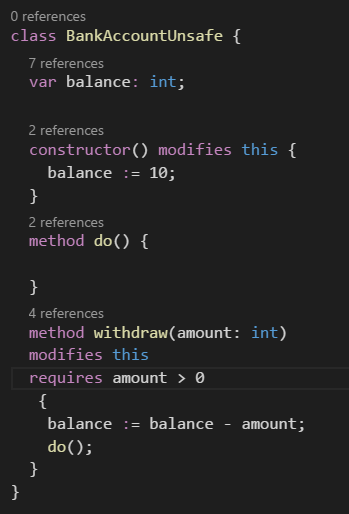
\includegraphics[width=0.5\textwidth]{img/codelensesClosed}
	\caption{Code Lenses used with Dafny}
	\label{fig:codelensesclosed}
\end{figure}

The first decision to be made was for which elements in the code codelenses should be displayed. The adeoff here is to  provide enough information to work comfortably with the codebase and not to clutter the workspace with codelenses. It was decided to display codelenses for classes, methods (including constructors) and fields, since they tend to have a wide scope in the codebases. \newline
A second consideration was which information should be displayed in the codelens. When codelenses are language specific and do not for instance stem from a plugin which displays code metrics are similar, usually references and usages of the element are displayed. Since this allows the programmer to gain a deeper understanding of control flow and regions affected by refactorings, it was decided to display this information also for the Dafny plugin. Codelenses also allow commands to be executed when clicked upon, a logical conclusion is to implement go to reference when a reference in a codelens is clicked.\newline

\begin{figure}[H]
	\centering
	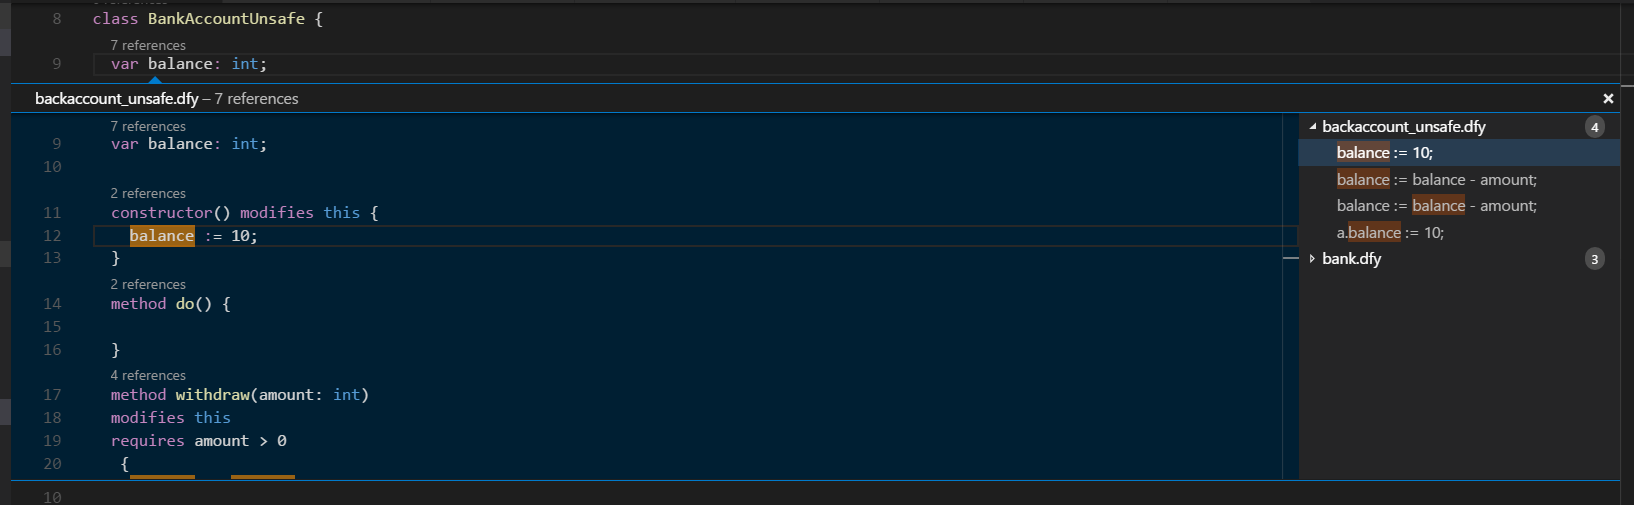
\includegraphics[width=1\textwidth]{img/codelensesExpanded}
	\caption{Expanded codelens showing the references to the field balance}
	\label{fig:codelensesexpanded}
\end{figure}

The only challenging aspect when implementing this feature is that references can't be determined via a simple text search, since different classes could have member with the same name. To only display unambiguous references, the search has to be done via the fully qualified domain name of the symbol. Since information about references is needed often, all references are determined by the DafnyServer and returned together with the symbolinformation to the symbolservice. This allows for simple processing in the language server itself and the references are updated in real time, since the symbolservice refreshes the symbols for a file when it is changed. Off course also the filepath belonging to the file in which the reference occurs is returned by the symbolservice. This is needed when a reference is a file external to the defining one and the go to reference command is invoked.\newline
When given locations of the references, it is possible to let visual studio code highlight them in the preview window which opens when a codelens is expanded. Visual studio code also groups references according to the filepath in the location, so the programmer gets to see a map of all references ordered by containing file to the right of preview window and can quickly navigating to them.

 \subsection{Code Completion} \label{codecompletion}
 Code completion has become a standard feature for IDEs. Microsoft calls it Intellisense in its products. It enables programmers to rapidly write code without having to keep all definitions in mind. Usually, when the programmer starts typing, a little popup appears where the programmer can choose options that complete the code he is currently writing. \newline
 
 Since this is arguably one of the most helpful features in IDEs, the implementation thereof was paramount to the completion of this project. \newline
 
 \begin{figure}[H]
 	\centering
 	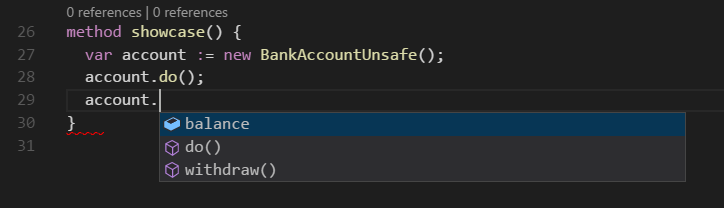
\includegraphics[width=1\textwidth]{img/codeCompletionOverview}
 	\caption{Popup with completion options}
 	\label{fig:codecompletionoverview}
 \end{figure}
 
 There are several different considerations when implementing code completion in a language server. The first one is to define which typed characters should trigger a completion request. Ideally, an IDE supports the programmer with completion regardless of the current context. Next to performance, another reason to narrow down the trigger selection is that not all contexts warrant meaningful suggestions for completion. In this project, a pragmatic approach was chosen where completion is triggered when ever a "." is typed, a situation where the programmer usually wants to access a member of an element. Since there is usually a designator present before the ".", there exists also enough knowledge about the current context to offer meaningful options. \newline
 In order to support this, the symbol service stores all variable declarations so the plugin knows about the type of all expressions that can be followed by a ".". The completion request comes with a position in the current file as an argument, so the first task is to resolve the expression and find out the fully qualified name of each element. The language server then searches the symbol service for all members that are defined in the class with that fully qualified name and sends them back as completion suggestions. \newline
 Visual Studio Code then handles all further actions, for instance, once the popup is displayed and the programmer continues to type, it removes all suggestions that don't start with the typed characters. It is also possible to display further information regarding the suggestions. The plugin already details if the completion is a field or a method, which Visual Studio Code provides own icons for. When the suggestion is a method, the preconditions, if any, are also displayed, so the programmer already knows the constraints he is writing under. \newline
 
 \begin{figure}[H]
	\centering
	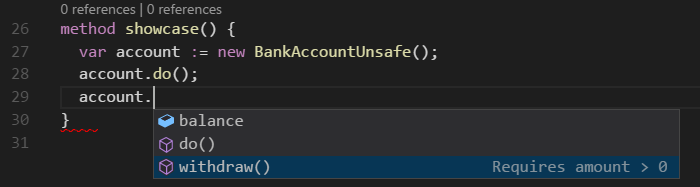
\includegraphics[width=1\textwidth]{img/codeCompletionMethod}
	\caption{Suggestion displaying precondition}
	\label{fig:codecompletionmethod}
\end{figure}

The implementation is straightforward, as the symbol service already provides ways to resolve the fully qualified name of an expression and if it as an alias for an element of a class, all therein defined methods and fields can simply be collected. The method and field symbols in the symbol services also contain all additional information which is displayed in the popup. Possible improvements in the completion feature would be support of built in methods and functions and also offer context aware completion when the programmer starts to type an identifier. 

\subsection{Go to Definition} \label{gotodefinition}
Another common feature in modern IDEs is go to definition. It enables the programmer to quickly jump to the definition of a code element he is currently working with to gain further insight about it. This can usually be done either via hotkey for the current cursor position or an option when opening the context menu via a right click, Visual Studio Code offers both ways.\newline
Since, similar to code lenses, this is a feature which is elemental to all modern IDEs and provides great overview over a project, the implementation of this feature had a high priority in this project. \newline
 \begin{figure}[H]
	\centering
	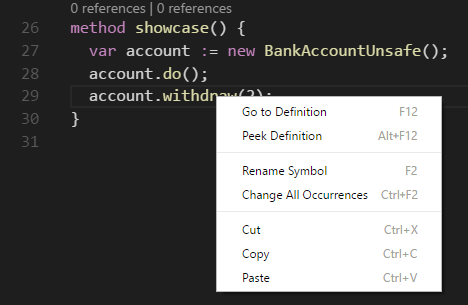
\includegraphics[width=0.5\textwidth]{img/goToDefinition}
	\caption{The Definition Features}
	\label{fig:gotodefinition}
\end{figure}
The language server protocol offers an on definition request, which has URI of the file and the position for which a definition is requested as parameters. The plugin language server then first tries to resolve the word at the position which could lead to a definition. When a word could be resolved, the plugin tries to determine if the expression is an alias for an element of a class or if it stands for an access of a member of one. If this is the case, the fully qualified name of the symbol can be determined via the symbol service, as it stores information about all definitions and declarations. The plugin than finds the unambigious definition via the fully qualified name and responds with the location of that definition. This also works if the definition is in an external file in the same workspace. \newline
If, for whatever reason, the fully qualified name cannot be determined, the plugin tries to match the selected word with any symbol cached in the symbol service. This approach only works as best effort though, as different classes could defines methods with the same name for example. If no match is found at all, no definition is provided. \newline
Visual Studio Code offers to options when searching for definitions, either go to definition which immideatly opens the returned location in an editor or peek definition, which shows the definition in a little overlay. \newline
 \begin{figure}[H]
	\centering
	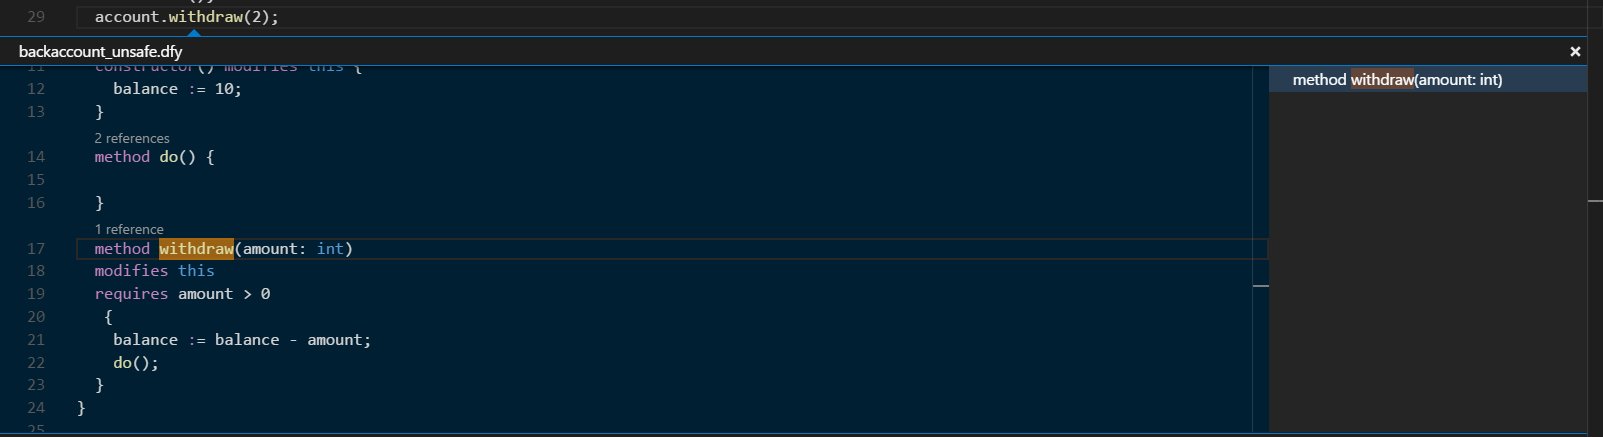
\includegraphics[width=1\textwidth]{img/goToDefinitionPeek}
	\caption{Overlay of peeked definition}
	\label{fig:gotodefinitionpeek}
\end{figure}
Extensions to this feature could be a context aware heuristic when a fully qualified name cannot be determined where for instance the current and nearby files are preferred when searching for definitions. Also, when polymorphism comes into play and the actual implementation cannot be determined, at the current state the first possibility is returned. The could be enhanced by offering all possible definitions.


\subsection{Rename Element} \label{renameelement}
Rename element is a feature essential to refactoring. It is widespread in IDEs and allows to quickly make code better readable Visual Studio Code offers built in support for renaming either via a hotkey or the context menu. \newline
Because of its importance in refactoring, which is one of the most important tasks when programming, implementing this feature belongs to the core scope of this project. \newline
The language server protocol, as with many other features, offers a request for renaming with the URI of the file in which the command was invoked and the position belonging to the command. Additionally, the new name the element should have is also given as an argument. The protocol expects a collection of textedit commands, which entail an URI of file, and ranges in that file which should be replaced with a word. \newline
As often with the language server protocol, the first step when implementing the feature is to determine the element at the position which is given as an argument. When the position can be resolved to a meaningful word, the plugin tries to determine if it is either an alias for an element of a class, or a member of class, for instance a field or a method. If it can do so with absolutely certainty, the fully qualified name of that element is obtained. The next step is trivial, since the symbol service already caches all references to a symbol, information which it gained through the DafnyServer. The plugin can simply build textedits out of all references, since the reference already contain all necessary information such as the containing file and their position therein. This therefor also works across multiple files which reference the same element, as long they are open in the same workspace. Those textedits are then returned from the language server to Visual Studio Code, which does all the actual replacing. \newline
  \begin{figure}[H]
 	\centering
 	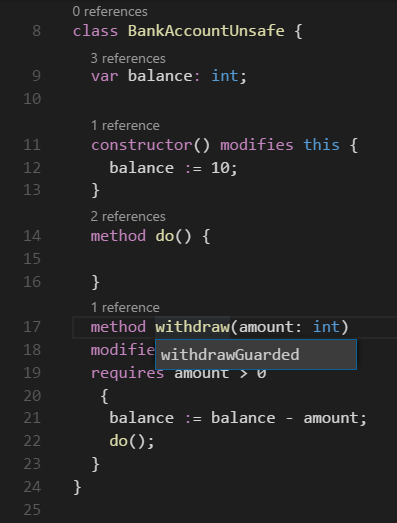
\includegraphics[width=0.5\textwidth]{img/rename}
 	\caption{Renaming an element in Visual Studio Code}
 	\label{fig:rename}
 \end{figure}
Since this feature acutally changes code that is worked with, the implementation must be very robust and failsafe. Thus, it was implemented very defensive. It the location of a requested renaming cannot be resolved to a meaningful word, the request is ended without dictating any changes. The same hold if a word can resolved, but it cannot be matched to a fully qualified name. In this case, possible references could be ambigious, so no action should be taken. To further limit the possibility for failure, the scope for this feature is very small. The current stand only allows for renaming of class members susch as fileds and methods, since these can be resolved with absolute certainty.\newline
When extending this feature, if would be benefical to also be able to rename local variables for instance. To do this, the symbol informtation which the DafnyServer returns to the symbol service would have to be enriched with detailed scope information to allow being able to exactly say which regions are prone to renamings and which are not. 
\subsection{Quick Fixes} \label{quickfixes}
Quick Fixes are a versaile feature in IDEs which basically allow to do any manipulation to code. Usually they are offered as reactions to diagnostics which were provided earlier. A simple example would be implementing a spell checker this way, offering to replace a wrongly written word with the correct spelling. \newline
Since this feature has no clear implementation guideline, and the plugin designer can implement almost anything that he likes this way, this was an obvious place to implement Dafny specific feature in the plugin. \newline
They this works in Visual Studio Code is, when the diagnostic stage for the file has been completed, where all things such as compiler warnings or custom warnings are generated,  a new request is fired at the language server. This request holds a collection of all diagnostics on the current file and the the language is free to either do nothing are provide commands for some diagnostics in the collection which often aime to resolve the shortcomings detailed by the diagnostic. \newline
  \begin{figure}[H]
	\centering
	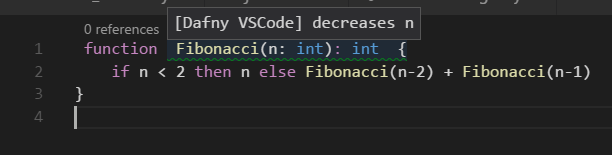
\includegraphics[width=1\textwidth]{img/diagnostic}
	\caption{Visual Studio Code displays a diagnostic}
	\label{fig:diagnostic}
\end{figure}
The current stand of the projects offers two code fixes to resolve Dafny specific diagnostics. \newline
The first one is a common situation where a programmer fails to capture his intention that a variable should either decrease or increase a variable when working with recursion or loops. The remedy is simple, a decrease guard with the variable in question must be added at the correct location. \newline
  \begin{figure}[H]
	\centering
	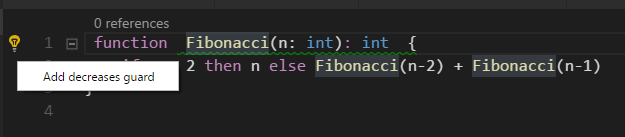
\includegraphics[width=1\textwidth]{img/decreaseGuard}
	\caption{Offering a code fix to add a guard}
	\label{fig:decreaseguard}
\end{figure}
This situation can easily be identified through the message within the diagnostic, since Dafny always gives this message in the same format. The expression that has to be decreased can also easily be parsed out of this message. A little more difficult is the placement of the guard, the implementation tries to find the first block in which the variable is not in scope anymore. The guard is then inserted before the block containing the first usage is used. \newline
  \begin{figure}[H]
	\centering
	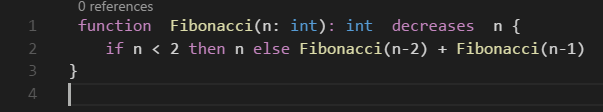
\includegraphics[width=1\textwidth]{img/decreaseGuardApplied}
	\caption{Programm after the code fix}
	\label{fig:decreaseguardapplied}
\end{figure}
The second code fix the plugin is offered is very similar, but this time the constraint is that an object may be null when it should not. The situtation again is easily detected through the message in the diagnostic, and also the expression which should not be null can be parsed through it.
  \begin{figure}[H]
	\centering
	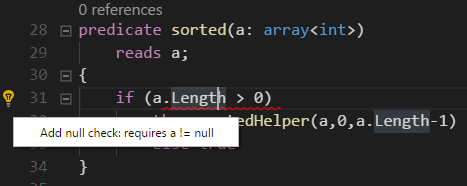
\includegraphics[width=1\textwidth]{img/nullCheck}
	\caption{It should be made sure that an element is not null}
	\label{fig:nullcheck}
\end{figure}
Also the search for the insertion position works very similary. It then inserts the constraint in form of a precondition of the sourrunding element. \newline
  \begin{figure}[H]
	\centering
	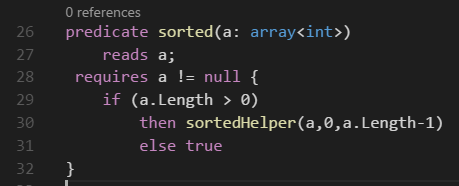
\includegraphics[width=1\textwidth]{img/nullCheckApplied}
	\caption{The precondition has been added}
	\label{fig:nullcheckapplied}
\end{figure}
At the current stand, only these two code fixes are implemented, the possible extensions are legion. 
\subsection{Environment}\label{environment}
This chapter details the underlying structure of the plugin which provides a basis to implement the individual concrete features.

\subsubsection{Symbol Service}\label{symbolservice}
The different features often need detailed information about symbols and their relations. A symbol table is a datastructure used by a compiler to keep track of scope / binding information about names. These names are used in the source program to identify the various program elements, like variables, constants, procedures, and the labels of statements.\cite[239]{compiler} \newline
With regard to performance, but also to reduce overhead it was decided to implement a symbol service in the language server part of the plugin. It's main goal is to cache a subset of the symbol table of the compiler, such that features which need information about names in the code can use the symbol service to gain this insight without having to invoke the compiler every time a lookup has to be performed or each feature having to handle the information caching seperately. \newline
Since compilation is a heavy task, results should be cached efficiently. There is a tradeoff here though with the validity of the symbols, since if they are cashed too long, they don't represent the code anymore. The solution chosen is a lazy loading approach, meaning whenever a component queries the service the first time, the symbols are cached the first time. This is usually done through the codelenses, since they need the symbol information and they are created every time a file is opened right at the start. To make sure that no unnecessary loads are performed, the symbol table for each document is stored alongside a hash of the content of the document. Before sending a new request to DafnyServer, a comparison of the hashes is done to acertain that the file really has changed. In future, this would also allow efficient caching by using histories of symbol tables when actions are undone. Next to the symbol table, it also stores the supplied textdocument itself, allowing for quick text manipulation if the content has not changed when loading the symbols.\newline
The next consideration was on how to store the symbol table and which information should be saved. The fields used are mostly needed to either determine which kind of symbol it is, where its scope is, its fully qualified name and relationsships in form of references are also stored. This lead to the following data structure that is stored in the symbol service, the example is simplified for better readability: \newline
\newline\newline
\textbf{Symbol Tables: }
\begin{lstlisting}[language=json,firstnumber=1]
[
 {
  fileName: "filepathInUriFormat",
  hash: -483616355,
  symbols: [
   {
    call: null,
    column: 5,
    document: "filepathInUriFormat",
    end: Range(8, 12),
    ensures: [...],
    line: 8,
    module: "module",
    name: "balance",
    parentClass: "BankAccountUnsafe",
    position: 96,
    range(start, end),
    References: [
     {
      column: 4,
      document: "filepathInUriFormat",
      end: Range(11, 11),
      line: 11,
      methodName: "balance",
      position: 154,
      range: Range(start, end),
      referencedName: "balance"
     },
     ...
    ],
    requires: [...],
    start: Range(8, 5),
    symbolType: "Field"
   },
   ...
  ]
 },
 ...
]
\end{lstlisting}

The possible symbol types that are stored are defined as follows:
\begin{lstlisting}[language=json,firstnumber=1]
{
 Unknown,
 Class,
 Method,
 Function,
 Field,
 Call,
 Declaration	
}

\end{lstlisting}
The symbol table offers the following API to obtain symbols: \newline
\paragraph{addSymbols(doc: Textdocument, symbols: SymbolTable, forceAddition: boolean=false): void} This saves the supplied symboltable and assocatiates it with the textdocument given. The default behaviour is to get a new symboltable from the DafnyServer anyway and compare if they have changed. If so, the never one is chosen and persisted. If the parameter forceAddition parameter is set to true, the symboltable is stored even though it might be out of date.

\paragraph{getTextDocument(uri: string): TextDocument} If the service has cached a textdocument specified by the uri supplied, it returns it.

\paragraph{getSymbols(doc: TextDocument): Promise<SymbolTable[]>} Returns all the symbol tables that are stored in the symbol service. Optionally, a textdocument can be given as an argument. If the symbols to this document are not cached, then they are queried from the DafnyServer. Since this is an async operation, the return type is a promise of symbol tables. This method is useful when actions have to be done across the whole workspace.

\paragraph{getAllSymbols(doc: TextDocument): Promise<Symbol[]>} Similar to the method above, but the result is already flattened to an array of symbols accross the whole code base. This is useful when it is not important to work with the symbols on a file per file basis.

\paragraph{getSingleSymbols(doc: TextDocument): Promise<SymbolTable>} This method allows for gaining the symbols for a single textdocument. If they are not cached yet, the service queries the Dafny Server for it, stores the result and then returns it. Since this operation is async, the return type is a promise.

When querieng the the DafnyServer, the server defensively starts the communitcation with it by supplying the symbols verb and the filepath and content for which it wants symbols on stdout. It then waits on the socket for a response, and if it is well formed and contains the queries symbols, the json returned by the server is parsed and then new Symbol elements are constructed out of the json, which are then saved in the service. \newline
When there is an error, for instance a connection error, or there was a compilation error which prevents the building of a symbol table, the service deals with the error and just keeps, if it has any, old symbol table of the file, so that the data is always in the most consistent state possible. Since compilation errors or connection errors are signaled to the user, the service listens until the broken elements have been repaired and then queries the server again for the symbols. \newline
Parsing of a successful response is also done conservatively, meaning that if an important property on for instance a method symbol is missing, this symbol is not stored, although all other valid symbols from that batch are stored. This allows for the maximum of analysis with only partly correct data. \newline
An improvement to the symbol service could be to do the caching more cleverely, for instance ignoring white space changes. A tradeoff in this area is that the calculations to decide if an update should be made could be more expensive then the update itself, so this should be monitored closely. Also when more and more complex refactorings and analysis should be done with the plugin, the data structure stored must probably be expanded. The extreme would be to save the whole AST in symbol service which off course would be overkill. Also here a blance thusly must be found between information richness and scope. Another consideration could be to optimize the lazy loading approach, for instance draw on a simple heuristic which files might be openend soon and load the symbols for them preemptively\newline



\section{Course of the project} \label{projectCourse}
This chapter details how the project was implemented and in what way it deviated of the project plan.

\subsection{Deviations from the project plan}

\subsubsection{UC3: Reporting of Dafny best practices violations}
While this idea seemed obvious when planning the project, this feature could sadly not be implemented. When working with different IDEs and well established programming languages, a programmer is often used to be supported by tools which can help write cleaner and more idiomatic code, such as linters. From this viewpoint, the integration of such a tool into the plugin seemed necessary. \newline
While established languages have a pool of agreed upon best practices, Dafny is still a very young language with not yet wide spread usage. The tooling around Dafny is also still not as sophisticated yet as for other languages. From this it can be inferred that there is not yet a big collection of programs to gain experience from, and that the problem of establishing a clear work flow with Dafny usually still exists, further preventing programmers to concentrate on idioms. \newline
These facts reflect why there is no collection of best practices for Dafny yet, either in form of some documentation or as a suggestion from people that are involved with Dafny. \newline
A second point worth noting in regard to this use case is how best practices for Dafny could look like. Dafny differs to most other languages in that it provides excellent specification constructs. A natural area to agree on idioms would therefor be the contracts of a piece of code. This could also greatly enhance the performance, because if clever usage is made of techniques such as short circuiting, a proof can be calculated at a much lesser cost than with a naive implementation. \newline
While providing support for best practices for contracts would therefor be very nice, this would also be almost unsolvable complex. Even for simple cases a deep understanding of proof theory would be needed, while for complex conditions it is not determinable if they can be proven in a better way or if they can be specified and proven at all. \newline
Since the establishment of own best practices for Dafny without being able to include an existing collection was deemed an unrealistic, and the structuring of contracts in the best way possible an unsolvable task, it was decided to concentrate on other features of the plugin instead. \newline


\subsubsection{UC4: Automatic generation of contracts}\label{missinguc4}
Since the biggest selling point of Dafny is the possibility to write specification constructs. It therefor was clear to try to provide automatic generation of some of such constructs in this project. While planning the project, the proof pipeline used by Dafny was not yet understood fully, the grasp on proof theory was quite small as well. This made it very hard to estimate if such a feature could be implemented at all and if so, in what time. Nevertheless the potential benefit of such a feature marked it as a milestone in this project. \newline
While researching the theoretical basis for implementing such a feature as detailed in \ref{examples} and the chapters following it, it became apparent that the topic was quite complex. A first stumbling block were invariants. As languages such as Eiffel \ref{eiffel} make it is to work with invariants, it was assumed that Dafny offers this possibility as well. \newline
As was learned, there are several different methodologies when it comes to invariants, having them implemented as a macro which simply inserts them as postconditions to every block is simply the easiest approach. A collection of techniques can be found in \cite{invariants}. 
Dafny doesn't build in object invariants because it doesn't commit to a particular methodology. Since the upholding of certain business rules (which was the aim of this use case) via specification constrains usually translates into generation of invariants, in addition to generating the invariants, it would have also been in the scope of this project to define how to deal with invariants in Dafny in a consistent work. It was also impossible to define and implement a way in which such business rules could be expressed regarding time and the trade off between usability and flexibility.\newline
The second idea was to apply the concept of the weakest precondition. This means that if a proof does not hold given a context, one can find the weakest precondition to make the proof valid. It would have been great to offer the generation of the weakest precondition as a refactoring in the plugin. However, since the weakest precondition must be expressed in Dafny, it would have to be found in almost human readable form. Z3 \cite{z3}, the theorem prover used by Dafny, tries to prove a theorem via contradiction, it is very hard to gain information about satisfiability from the prover. Additionally there is the problem that Dafny code gets translated to the Boogie\cite{boogie} meta language, which then gets translated to Z3 syntax. Even if one could gain information from Z3 about satisfiability, it would therefor be difficult to provide a matching back to the Dafny language and display this information. In general, the problem of inferring sufficient conditions for proofs is very hard if they should be human readable, the few existing solutions work with an iterative approach relying on stepwise reduction of counter example, for instance described in \cite{preInference}. This approach is difficult to implement and lacks the usability that was sought after in this use case.\newline
Lastly, it took a lot of time to gain a working knowledge of the proof pipeline. Since it consists of three big projects, namely Dafny, Boogie \cite{boogie} and Z3 working together, a deep understanding was not possible without having some existing knowledge in this time. While trying to understand the pipeline, it also became apparent that the knowledge of the authors in proof theory was not deep enough to really grasp the problem and work on a solution in a feasible time. \newline
Because of all these reasons, it was decided to not implement this use case in this project. While this is regrettable, other ideas were gained during the investigation of the problem. The feasibility of displaying counter modules was discovered, as well as small refactorings that provide constraints for a small, but very often needed set of instructions such as array accesses were thought of. The remaining time of this milestone therefor was directed at implementing these features instead. 

\subsubsection{Code Actions}\label{addCodeActions}
As detailed in \ref{missinguc4}, while trying to implement a proof of concept for contract generation, some often used concepts while working with contracts were discovered. This led to the idea to offer refactorings to generate the correct contracts for these concepts. While this is in no way a generic approach towards contract generation, it seemed as though these refactorings could help in many situations, making life considerably easier for the programmer. It was therefor decided to implement them, partly replacing the goals sought after in use case 4. A more complete picture, including an overview of the implementation, can be found in \ref{quickfixes}. The following list details on why these concepts were chosen. \newline
 
\paragraph{Null Check}
Programmers very often access members of elements, especially in the methodology of object oriented programming. While it offers a great way to structure a program and to represent reality in a program, it comes with some danger. The most common pitfall is what Hoare famously declared his biggest mistake\cite{hoare}, the null reference. To help avoid this, Dafny reports potential null reference. Since almost any piece of complex code deals with objects, this is a very common occurrence, since for instance every object given as an argument must be checked for null first. \newline
It was decided to offer a mitigation of this important, but tedious work. The plugin detects warnings about potential null references, and offers to generate a precondition that demands that the designator standing for the potential null reference may not be null. If the programmer accepts the proposal, the precondition is inserted at the correct location. This shifts the burden of providing a valid context to the caller of the method, so the method can concentrate on offering a solution to the call. While working with Dafny, it was noticed that such a precondition was needed for about every third method, meaning that a lot of work is done for the programmer by supplying this precondition generation.
\paragraph{Bound Checking}
Almost as often as checking for null, it is necessary to check if an index to an array is in bound. Dafny already has sufficient knowledge about the array data structure that it issues a warning every time it is not clear if an index that is used to access an element is in bound of the array. While programming with Dafny, it was observed that this is the case in almost every non trivial example using arrays. Since the array data structure is used quite often in Dafny, it was decided to also help the programmer with this construct, since bound checking is important, but tedious. \newline
Whenever a warning is issued by Dafny that an index may be out of bound, the plugin offers to generate two preconditions, namely one that states that the expression representing the index must be bigger than zero, and one that states it must be smaller then the array length minus one. The placement off course must be so that the preconditions are introduced at a place in the program where all variables used in the expression have been declared. When the programmer decides to use the quick fix, the preconditions are inserted and relieve him of the hassle of manually checking the bounds of the index.
\paragraph{Increase / Decrease / Invariant Guards}
Another concept that often arises when using Dafny is to make sure an expression converges to a certain range of values over time. This is the case when making use of recursion to ensure that the base case is eventually met, or when writing loops that depend on a certain value of an expression for termination. Both examples are very important, because not handling them correctly can result in endless loops or overflow. Dafny already does a good job in generating warnings that tell the programmer that constraints should be enforced for a certain expression. \newline
These situations also occur very often, since both recursion and loops are fundamental elements of programming, it was decided that the generation of these constraints could greatly benefit the programmer. In order to do this, the plugin offers to add an increase / decrease clause with the correct expression in place when Dafny detects recursion or a loop. When the programmer chooses to use the quick fix, the guard statements are inserted at the correct place. Another important constraint when working with loops goes hand in hand with the use case described above, namely when an array is accessed within a loop and the expression used as an index is not constant within the context of the loop. For this, Dafny offers the construct of invariants, that ensure that an expression is within a certain range during a given context. The plugin therefor offers to generate invariants which ensure that an expression used as an index is always in bound of the array. When the programmer chooses to use this feature, the invariant is inserted at the correct context. 

\subsubsection{Counter Examples}
A concept which was not known as the project started, were counter examples. They provide a huge benefit, as to understand how a program violates its contract. Especially if it is a more complex software with many methods and many branches, it can be very difficult to understand why a contract does not hold\newline
For this reason it was decided to implement that features in addition to CodeActions \ref{addCodeActions}. 
Developers can use this practical features directly in Visual Studio Code. It shows on each line how the variables have to be assigned that the proof fail. \newline
Because the calculation of the model, how it is called in Z3, can take very long, it is not run automatically if a proof fails. Nevertheless this can be overridden over the configuration. 
 
\subsubsection{Displaying Control Flow}
\todo{Add}


\section{Possible points for Extension} \label{extensions}
This chapter details what further work could be done on the plugin by subsequent projects.

\subsection{Support for other IDEs} \label{ides}
Since the plugin is structured as a language server, it should theoretically be possible to integrate it into any IDE which implements the language server protocol without any problems. In reality, some customization is often needed and some popular IDEs also do not fully implement the protocol yet. This chapter details which IDEs were looked at as possible hosts for the plugin and what would have to be done for a complete integration.
\subsubsection{Eclipse integration}
The eclipse project \href{https://projects.eclipse.org/projects/technology.lsp4e}{LSP4E} aims to integrate existing language servers into the Eclipse IDE in an easy way. 
\newline
"It includes some APIs to turn language server protocol elements into Eclipse IDE concepts and a generic integration allowing to easily plug any language server to an Eclipse IDE instance without need to write Java code, either via a plugin associating a new language server, or by letting users manually bind language servers to their IDE." \cite{lsp4e}
It is built on top of \href{https://github.com/eclipse/lsp4j}{LSP4J}, a Java implementation of the language server protocol. 
\newline
Integrating the Visual Studio Code Dafny language server into Eclipse could become possible in the future. Right know there is no way to interact on the client side. One only can specify a language server based on a program (NodeJS) and arguments (extension.js) which is executed and used for querying information. One cannot add any behavior to Eclipse itself, which would be necessary for certain features. Also, the sendRequest protocol specification is not implemented yet (Commit: 1615e07), which is important for starting the DafnyServer correctly. 
The better way would be to program a new Eclipse plugin, based on LSP4J, which then would also allow to customize the status bar, run scripts and show progress information. 
\subsubsection{Emacs integration}
Emacs \cite{GNU} is a versatile IDE which enjoys great popularity especially in the open source community. Written in LISP, Emacs traditionally supported language integration via so called modes, which are demons that run in the background. This is already a similar architecture as used in a language server integration. \newline
Work on integrating language servers into Emacs has already be done. The project emacs-lsp \cite{emacsLsp} aims to provide the connection between Emacs and language server. The project itself is structured as a classical Emacs demon and allows interactions with a language server. There already exist some integrable language servers in languages such as Java or Haskell. The integration of emacs-lsp and existing language servers seems to be pretty trivial, an example can be seen in \cite{javaEmacs} using Java. \newline
Since the language server allows custom messages to be defined as detailed in the implementation documentation, the Dafny plugin defines some of them. One set of custom messages is necessary, since the plugin allows for downloading the Dafny compiler automatically. The communication in regard to this feature must be extended to the IDE, so that the user is aware of this feature. Additional custom components are the state of the file so that the programmer sees if it is verified or not, or the displaying of counter examples for proofs.\newline
These features were deemed very useful in this project, such that they should be a part of every IDE integration. This means that a little wrapper would have to be written on the client side of the language server, which understands the custom messages and can relay this information to the IDE itself. The work that has to be done is trivial, since it simply means to pass information on and display them accordingly. \newline
It was decided that gaining a working knowledge of LISP and Emacs in order to write such a wrapper was not in the scope of this project. For a programmer familiar with Emacs and LISP this task should take no more than a week. The custom messages that need to be implemented can be found in the implementation documentation. It can be argued that this extension should be one of the first ones to be tackled by later work, as one can gain a considerably larger user base without having to invest too much work. 
\subsubsection{Monaco integration}
Monaco\cite{monaco} is the code editor that powers Visual Studio Code. It is also possible to use Monaco as a standalone editor in the browser. It would be interesting to integrate Dafny directly into Monaco, since there are not many simpler setups imaginable as opening a browser window. It was therefore decided to look into a possible integration of the plugin during the course of this project. \newline
It soon became apparent that the project does not seem very active, as the latest commit was two months old at the time of this writing. The documentation for developers is also very sparse. There was hope that an integration would be trivial, since the plugin is structured as a language server. However, Monaco does not implement the language server protocol. In the documentation, it can even be read that "Extensions written for Visual Studio Code will not run in Monaco"\cite{monaco}, without any further explanation given. \newline
However, integrating a new language into Monaco is possible, as can be seen in an example for Typescript in  \cite{monacoType}. However, the setup is different than a language server integration or a Visual Studio Code plugin. It is questionable how much code could be shared. While the idea of running Dafny in an editor in the browser is interesting, the work that would have to be done in order to achieve this was deemed to be outside of the scope of this project. In addition, if further work aims to implement this integration, an evaluation on how active the work on Monaco is should be done first, given the apparent standstill in the project at the time of this writing.
\subsection{New Features} \label{featureExtensions}
This section details some interesting ideas that were gathered during development of the plugin, but were sadly out of scope of this project. It is thought as a starting point for developers that want to extend this plugin. 
\subsubsection{Debugger}
Integrating a debugger into the plugin would be great, since this is a feature that is very often used and very helpful when searching for bugs. An existing solution already support this feature, namely the Visual Studio integration \cite{visualstudiodafny} of Dafny. This already works very well and can be used as a guideline when developing an own integration. It is also a feature that programmers have become used to in all modern IDEs so it should be part of any language integration. \newline
Sadly it is also quite a difficult task since the interaction between an IDE, an executable and a debugger is complex. While the Visual Studio integration is open source, it is written in C\# and can therefore interface directly with the Dafny pipeline, which is heavily done in that integration. It would take quite some work to abstract this direct interaction into a clean API that extends the existing API of the Dafny pipeline. Using this API, a language server could provide an own implementation of a debugger.\newline
Designing this complex component was well out of scope for this project. It is estimated that, depending on the preexisting knowledge, this would be an endeavor of about two to four weeks time and probably would have to rely on at least some help by the Dafny development team. While this task is difficult, the result would be having an important feature that all users of modern IDEs anticipate in a language integration. It therefor should be a primary consideration when deciding on how to extend this project. 
\subsubsection{Widening Scope}
While many features have been implemented during the course of this project, the scope of their application was often narrowed as to provide a pragmatic approach to the problems regarding the scope of the project. For example, the rename element refactoring only works on members of classes, but not on parameters of methods. \newline
The exact scope of all features can be found in the API documentation of this project. While the extension of scope of existing features might seem tedious and not very interesting, it can introduce subtle problems that have to be dealt with with great care. It also is benefical to the users, as they can apply features in much wider contexts. 
\subsubsection{Contract Generation}
While contract generation has been implemented for some often occurring situations as detailed in \ref{dffeatures}, there is still a big potential for improvement in this area. Since a generic approach to contract generation has been deemed to be unfeasible, the next best way is to offer help in writing specification constructs in specific situations.\newline
When deciding to do work in this area, it is important to first analyze which situations appear often in a typical Dafny program. While this task it is difficult in itself, since it requires some expertise in Dafny, it is important because otherwise features may be implemented that do not get used in every day scenarios. \newline
When such situations have been identified, the specification construct generation must absolutely be correct. Since this is a feature that changes existing code, it is better to not provide any help when there is ambiguity regarding the correct solution. However, when done correctly, this is a feature from which programmers can greatly benefit, since it enhances productivity by eliminating the need to do complicated reasoning. It also introduces capabilities of Dafny to programmers that are not yet proficient in their usage of the language.



%\section{Ergebnisse}
[Placeholder]
%\section{Ausblick}
[Placeholder]

\appendix

\listoffigures
\addcontentsline{toc}{section}{\listfigurename}

\listoftables
\addcontentsline{toc}{section}{\listtablename}
\printbibliography[heading=bibintoc]
%\section{Anhang}
[Placeholder]
\end{document}
